% Chapter 2

\chapter{State of Art}
\label{Chapter3} 

\section{Device}
The personal health care market has changed a lots and recently new products and devices are showing up on the market. We will describe briefly the most relevant and similar products as mobile ECG acquisition devices.  We evaluate the following solutions:
\begin{itemize}
	\item Mortara ELI 10 Mobile
	\item Philips DigiTrak XT Holter Recorder
	\item M-Trace (PC) Mobile
	\item ECG Expert 
\end{itemize}

\subsection{Mortara ELI 10 Mobile}
This device offers an all in one solution for 12 leads ECG acquisition. It is compact and complete as it provides an alphanumeric keyboard and a screen for real time visualization and the possibility to send the record via GPRS/3G channels. For each devices a SIM card is required . The device can also read and interpret the ECG supporting the doctor. Interesting feature is its great interoperability with the main ECG data management systems.
\begin{figure}[ht!]
	\centering
	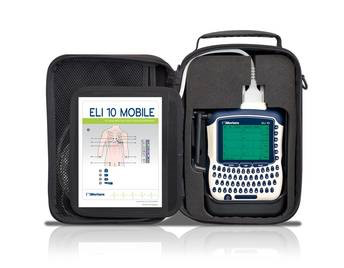
\includegraphics[width=90mm]{figures/ch3/1.png}
	\caption{Mortara ELI 10 Mobile, ECG acquisition device box.}
	\label{fig3.1}
\end{figure}

\subsection{Philips DigiTrak XT Holter Recorder}
This is the smaller acquisition device on the market. Thanks to a proprietary algorithm from Philips it can derive all the 12 ECG leads using only 5 leads. It weighs 62g and the internal battery lasts till 7 days. It also has a small screen showing 1 real time signal at a time.
\begin{figure}[ht!]
	\centering
	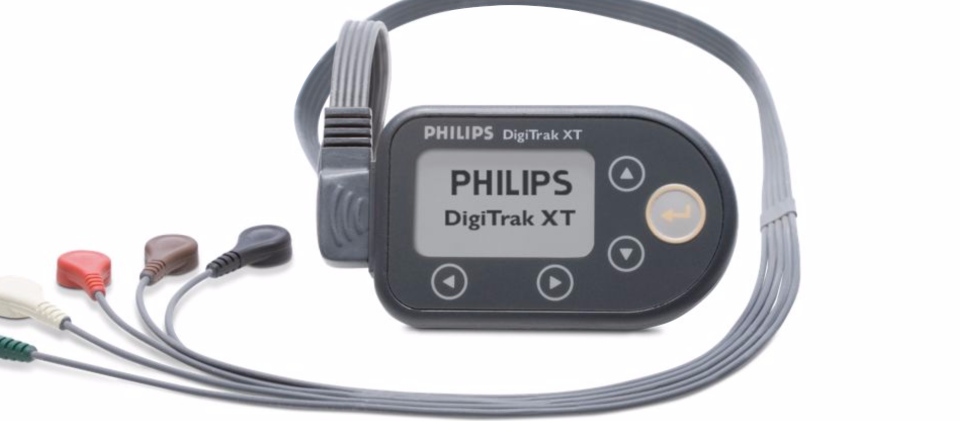
\includegraphics[width=90mm]{figures/ch3/2a.png}
	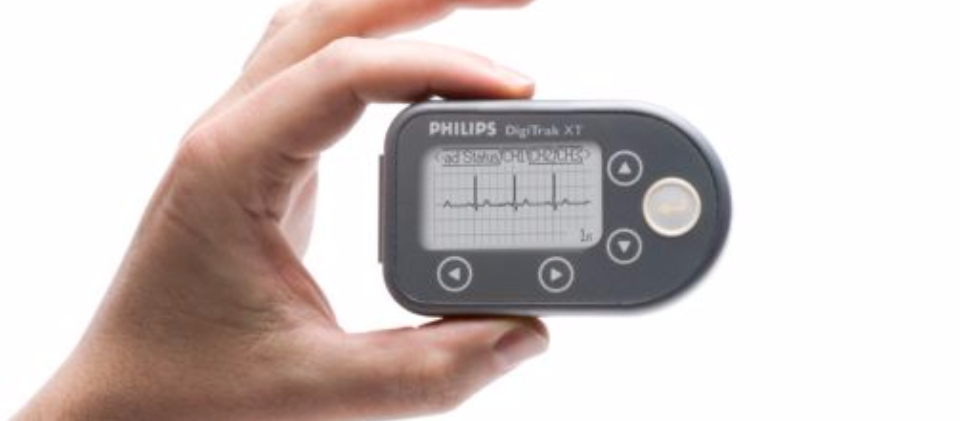
\includegraphics[width=90mm]{figures/ch3/2b.png}
	\caption{DigiTrack, the ECG visualization.}
	\label{fig3.2}
\end{figure}

\subsection{AliveCor ECG}
An innovative solution even though it doesn’t offer a complete solution for ECG acquisition and analysis. This small sensor can be attached on the back of your smartphone making it an ECG acquisition device. It can record only one ECG signal (D1), so also the analysis is limited to a few types of arrhythmias . The record length is also limited to 5 minutes.
\begin{figure}[ht!]
	\centering
	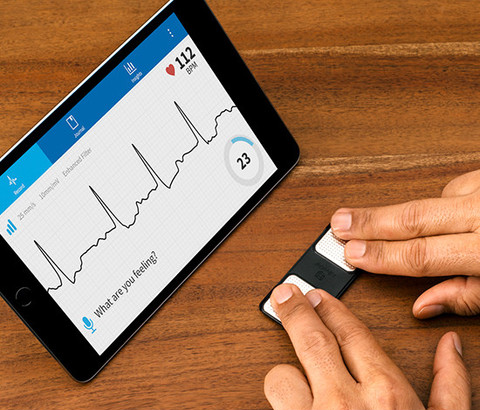
\includegraphics[width=90mm]{figures/ch3/3.png}
	\caption{AliveCor device real time acquisition on a tablet.}
	\label{fig3.3}
\end{figure}

\subsection{M-Trace (PC)Mobile}
M-Trace PC is an completed 12 leads ECG acquisition device. With the device it comes a mobile application and a desktop pc application used to visualize and analyze the ecg signals. The device is really portable with dimensions 95x64x28mm.  The company offers also a more portable device (M-Trace Mobile) to be used by privates at their home. The mobile version cannot acquire a full record but only test records with 6 leads. Its main purpose it to send the test records via GSM/GPRS to the doctor for a faster review.
\begin{figure}[ht!]
	\centering
	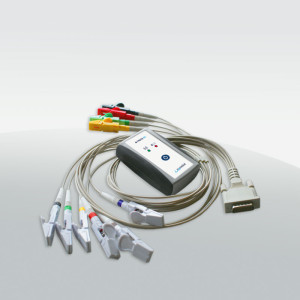
\includegraphics[width=60mm]{figures/ch3/4a.png}
	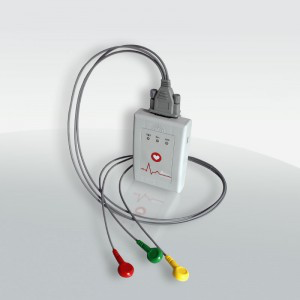
\includegraphics[width=60mm]{figures/ch3/4b.png}
	\caption{M-Trace PC device for ECG acquisition.}
	\label{fig3.4}
\end{figure}

\subsection{ECG Expert}
ECG Expert produced by CSE Medical is a completed solution for ECG acquisition. The device comes with fully supported software for both PC desktop (Windows and Mac) both smartphones  (Android, iOS). The device is rechargeable and makes use of a wireless connection via Bluetooth as exchanges data communication with the handheld smartphone or PC software.
\begin{figure}[ht!]
	\centering
	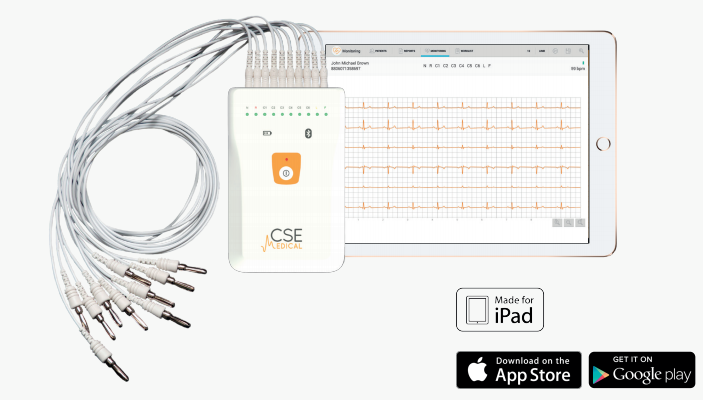
\includegraphics[width=60mm]{figures/ch3/5.png}
	\caption{M-Trace PC device for ECG acquisition.}
	\label{fig3.5}
\end{figure}

\section{Mobile application}
There are already mobile applications on the market store for ECG visualization and analysis supporting different formats. We can distinguish applications that only visualize the signal and the ones that also apply some analysis on the ECG signals. We listed only applications on the Google Play Store, so only Android applications because they are the only comparable with the solution we propose.

\subsection{Visualization only application}
The application on the market able to visualize the ECG signal are:
\begin{itemize}
	\item \textit{StribogECG}: an Android application based on an open source project under GLP v3 licence. It uses Biosig library to read ECG formats such as scp, xml (hl7), ecg and dgf. The software is only provided as it is and it requires to the user to already have the ecg files stored in those supported formats.
	\item \textit{AndroidECG}: application on beta release, it was developed by Paco Gonzàles as thesis project during the Master course in Computer Science at the University of Murcia. The application is able to show ECG signals of the following formats: binary, scp, 212. As additional feature it is a basic analysis over the signal to detect QRS complex, P waves, ST segments and T waves. It is also possible to send the ECG record via email.
\end{itemize}

\subsection{Visualization and Analysis}
The applications on the market that also provide a more detailed analysis over the ECG signal are all bind to a specific proprietary acquisition device. By this way they lack the compatibility and interoperability requirement with other software and ECG formats.
\begin{itemize}
	\item \textit{M-Trace PC}: the application was developed by \textit{M4Medical}, a Poland company providing medical devices for professionals and private customers. The application only works with the company 12-channel ECG M-Trace PC register device. The main features are the real-time monitoring interface, a patients’ database management system and the possibility to share the record.
	\item \textit{ECG Expert}: developed by \textit{CSE Medical} the application works only connected to an ECG-Expert acquisition device. The main features are the real-time view of the acquisition, the analysis of the record providing information about QRS complex and heart rate, the possibility to manage patient information bind to the record and a heartbeat Normal/Abnormal classifier.
\end{itemize}
One last mobile application, which is not strictly related to ECG signal visualization and analysis but it worth to be mentioned, is the \textit{ECG Interpretation}. This application instead provides  enough detailed information about how to read and interpret the ECG signals through 32 small lectures. All the lectures provide a picture and a short description and explanation.